\section{Test equation for ODEs}
Considering the test equation

$$
\dot{x}(t)=\lambda x(t), \quad x(0)=x_{0} \label{eq:test}
$$
for $\lambda=-1$ and $x_{0}=1$.

\subsection{Analytical solution}
It is is function that differentiated gives itself times a constant. Therefore for optaining the analyical solution, try a guess with:
$$
x(t) = \exp(\lambda t)
$$
Then
$$
x'(t) = \lambda \exp(\lambda t) = \lambda x(t)t  \quad \qed
$$
I.e. the analytical solution is $x(t) = \exp(\lambda t)$.

\subsection{Local and global truncation error}
In order to calculate the local and global truncation error, the exact, analytical solution to the ODE is required to be known. For that reason, the \textit{test equation} is typically used to \textit{test} the performance of numerical methods. The errors are calculated as follows \cite{JrgensenScientificEquations}:

\textbf{Global error}
$$
e_{k}=x_{k}-x\left(t_{k}\right)
$$
where $x_{k}$ is the numerical (descretized) solution and $x\left(t_{k}\right)$ is the exact (continuous) solution. The global error is thus the accumulated error over time. Therefore, it is commonly calculated in the last step.
\\

\textbf{Local error}
$$
l_{k}=x_{k}-x_{k-1}\left(t_{k}\right)
$$
where $x_{k}$ is the numerical solution and $x_{k-1}\left(t_{k}\right)$ is the analytical one-step solution starting from $x\left(t_{k-1}\right)=x_{k-1}$. Therefore, it is commonly calculated in the first step.
\\

\subsection{Computation of local and global truncation erros}

Now, it is of interest to calculate the error of the following three numerical methods
\\

\textbf{Explicit Euler \cite{JrgensenScientificEquationsb}}
\begin{equation}
    x_{k+1}=x_{k}+\Delta t f\left(t_{k}, x_{k}\right)
\end{equation}

Which intuitively takes a step forward with the current $\dot{x}(t_k)$.
\\
\textbf{Implicit Euler \cite{JrgensenScientificEquationsb}}
\begin{equation}
    x_{k+1}=x_{k}+\Delta t f\left(t_{k+1}, x_{k+1}\right)
\end{equation}

Which intuitively takes a step backward with the following $\dot{x}(t_{k+1})$ as estimated by Newton's Method [ibid.].
\\
\textbf{Classical Runge-Kutta \cite{JrgensenRunge-KuttaEquations}}
$$
\begin{aligned}
T_{1} &=t_{n} & X_{1} &=x_{n} \\
T_{2} &=t_{n}+\frac{1}{2} h & X_{2} &=x_{n}+h \frac{1}{2} f\left(T_{1}, X_{1}\right) \\
T_{3} &=t_{n}+\frac{1}{2} h & X_{3} &=x_{n}+h \frac{1}{2} f\left(T_{2}, X_{2}\right) \\
T_{4} &=t_{n}+h & X_{4} &=x_{n}+h f\left(T_{3}, X_{3}\right) \\
 t_{n+1}=t_{n}+h & & \\
 x_{n+1}=x_{n}+h &\left(\frac{1}{6} f\left(T_{1}, X_{1}\right)+\frac{1}{3} f\left(T_{2}, X_{2}\right)+\frac{1}{3} f\left(T_{3}, X_{3}\right)+\frac{1}{6} f\left(T_{4}, X_{4}\right)\right)
\end{aligned}
$$

Which intuitively takes a full step forward by taking 4 well-timed middle steps and calculating a weighted-average of those.
\\

The results are illustrated in the following two sections.






\subsection{Local error}
From Figure \ref{fig:1_4} it is clear that the Classical Runge-Kutta method is much more precise (on the test equation). In terms of order, a method is said to be of order p if $l_{k}=\mathcal{O}\left(h_{k}^{p+1}\right)$ \cite{JrgensenScientificEquationsc}. The \textit{order} is referring to the number of terms in the Taylor-expansion used to approximate $x_{k+1}$ from $x_k$.

By calculating the slopes of the linear line in the log-log plot we obtain:
$$
a_{Exp} = 2.00, \quad a_{Imp} = 1.98, \quad a_{RK} = 5.00
$$

Corresponding to orders
$$
p_{Exp} = 1, \quad p_{Imp} = 1, \quad p_{RK} = 4
$$


\begin{figure}[H]
    \centering
    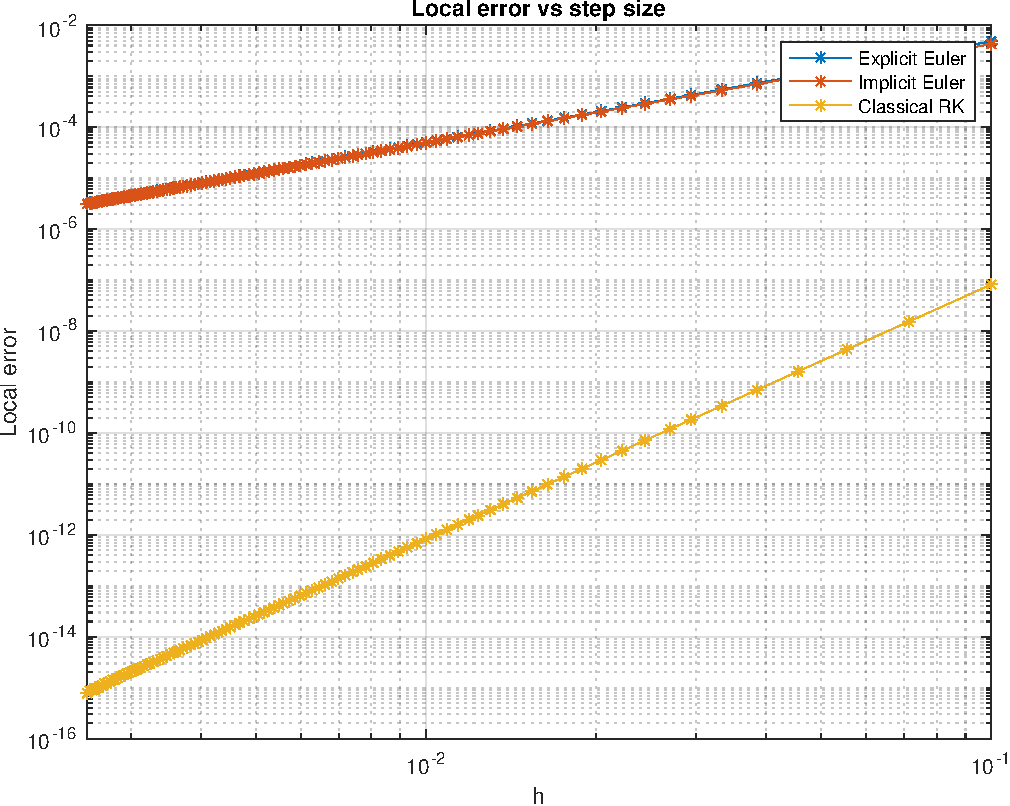
\includegraphics[width=0.7\textwidth]{plots/1_4.pdf}
    \caption{Local error vs step size for three numerical ODE solvers.}
    \label{fig:1_4}
\end{figure}



\subsection{Global error}
Similarly, the global error at $t=1.0$ for the three methods is seen in Figure \ref{fig:1_5}.

\begin{figure}[H]
    \centering
    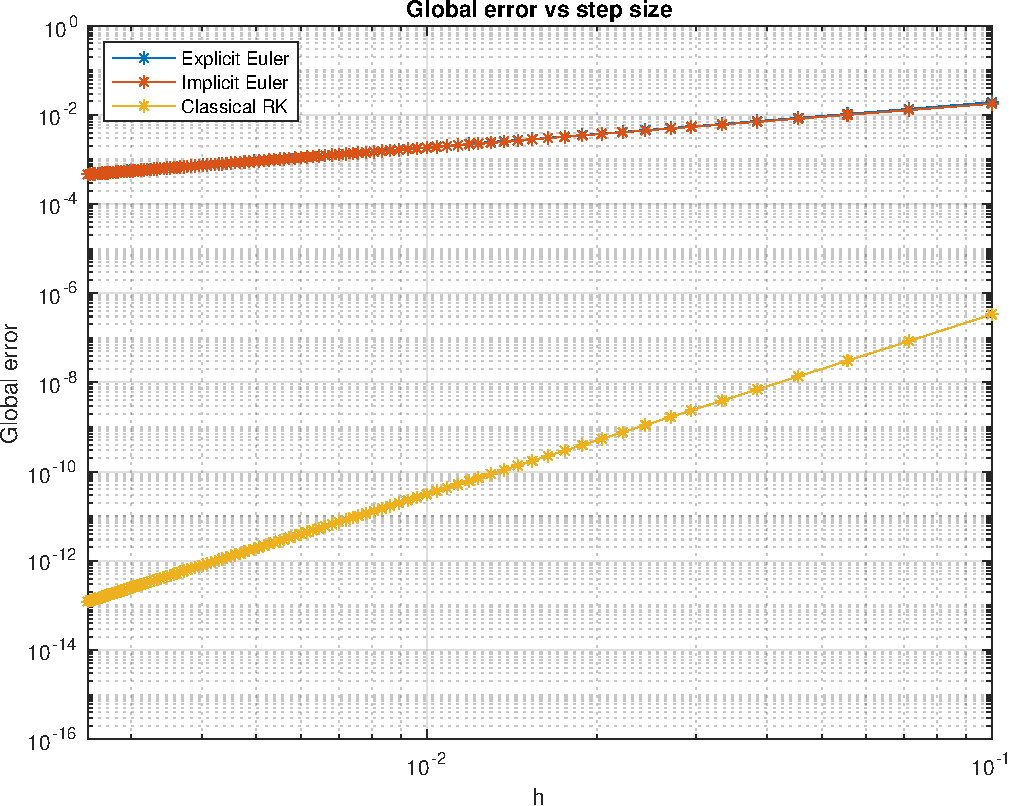
\includegraphics[width=0.7\textwidth]{plots/1_5.pdf}
    \caption{Global error vs step size for three numerical ODE solvers.}
    \label{fig:1_5}
\end{figure}

Again a close to identical performance is seen for the two 1st order methods with the Classical Runge-Kutta being much more accurate. The slopes are

$$
a_{Exp} = 1.00, \quad a_{Imp} = 0.99, \quad a_{RK} = 4.01
$$

Clearly, the global error is proportional to $h_{k}^{p}$, whereas the local error was proportional to $h_{k}^{p+1}$.

\subsection{Stability}
Stability of a methods relates to the \textit{transfer function} $R(z)$ in

\begin{equation}
    x_{k+1}=R(z) x_{k}
\end{equation}

The \textit{stability region} is then defined as \cite{JrgensenScientificEquationsc}
$$ \mathcal{D}=\{z \in \mathbb{C}:|R(z)|<1\} $$

Where $z = \lambda h$, such that if $R(z) > 1$ the method is unstable because the approximation $x_{k+1} \to \infty$ for $k \to \infty$ which is particularly erroneous for cases where $\lambda < 0$ of which the test equation is strictly decreasing. This later case is more formally called \textit{A-stable} [ibid.].

So for a method to be\textit{ A-stable}, it is has to fulfil \cite{JrgensenRunge-KuttaControl}:
\begin{equation}
    \forall z \operatorname{Re}(z)<0  :   |R(z)|<1
\end{equation}

In other words, the method is A-stable if there for all values of z where the real part is below 0 (\iff $\lambda < 0$ since the step size $h > 0$) the \textit{transfer function} is (numerically) below 1.
\\

For a method to be \textit{L-stable} it additionally has to fulfil:
\begin{equation}
\lim _{z \rightarrow-\infty}|R(z)|=0
\end{equation}

I.e. the \textit{transfer function} goes towards 0 when the step size times $\lambda$ goes towards -$\infty$.

\subsubsection*{Deriving stability regions}

Explicit Euler:

Implicit Euler

Classic Runge-Kutta:

[INSERT NOTES MANGLER]


\subsubsection*{Illustrating the stability regions}
The stability regions of the three methods is illustrated in Figure \ref{fig:figure3}. Referring to the definitions above it is seen that none of the methods are A-stable - and thus neither L-stable [TRUE?].

\begin{figure}[htp]
\centering
\includegraphics[width=.3\textwidth]{plots/1_6b.pdf}\hfill
\includegraphics[width=.3\textwidth]{plots/1_6c.pdf}\hfill
\includegraphics[width=.3\textwidth]{plots/1_6a.pdf}
\caption{Stability regions of the three numerical methods.}
\label{fig:figure3}
\end{figure}